\chapter[A PROPOSTA]{A PROPOSTA}

Este capítulo apresenta a proposta do trabalho de conclusão de curso, exibindo detalhes da implementação a ser realizada acerca da arquitetura bem como o protocolo de comunicação dentro desta.

\section{Introdução}
Avanços tecnológicos e a criação de linguagens de programação, diferentes técnicas e paradigmas e outros conceitos relacionados ao desenvolvimento de software contribui para que a necessidade de interação entre estes elementos seja emergente, de modo a viabilizar a construção de sistemas cada vez mais robustos e inteligentes. Esta interação entre elementos de software não consistem de aplicações robustas que executam todas as suas atividades de forma independente de outras aplicações, pois cada vez mais diversos sistemas de software interagem com outros, podendo ser estes desenvolvidos tomando como base outros paradigmas ou escritos em outras linguagens de programação e utilizando-se diferentes técnicas.

A fim de suprir esta necessidade de interação entre sistemas diversos, foi criado um modelo arquitetural conhecido como Arquitetura Baseada em Serviços (ou \textit{Service-Oriented Architecture} - SOA). Este modelo arquitetural utiliza o conceito de serviço como uma unidade que representa uma funcionalidade do sistema, além de trazer consigo os conceitos de interoperabilidade, flexibilidade, extensibilidade e baixo acoplamento entre os diversos sistemas ou serviços.

Para este trabalho de conclusão de curso, a proposta consiste em desenvolver uma arquitetura baseada no modelo SOA para um ambiente virtual, propiciando que diversos trabalhos já desenvolvidos e também aqueles em desenvolvimento não sejam mais "engavetados". Por meio do uso do modelo arquitetural baseado em serviços, será possível integrar tais aplicações, ou serviços, de modo que estas possam trocar dados e fazer uso do serviço disponibilizado por outras, indepentemente das tecnologias utilizadas para o desenvolvimento das mesmas.

Também faz parte da proposta, o estabelecimento de um protocolo de comunicação entre as aplicações, bem como o padrão de comunicação a ser utilizado, uma vez que as aplicações produzidas por outros podem se comunicar de modo a se tornarem mais robustas e completas enquanto ferramentas.

Desta forma, será viável a disponibilização à sociedade, interna e externa à Universidade, de uma plataforma virtual que conterá os trabalhos realizados dentro da mesma, sejam oriundos de projetos de conclusão de curso, disciplinas ou projetos de extensão e pesquisa.

\section{Proposta de arquitetura}

\subsection{Requisitos}
A partir da necessidade identificada de disponibilizar aplicações que foram desenvolvidas, bem como aquelas que estão em desenvolvimento e que serão desenvolvidas, através de uma plataforma virtual único, algumas das principais características arquiteturais deste ambiente que influenciaram na escolha do modelo arquitetural para a construção da plataforma são:

\begin{itemize}
\item A comunicação entre as aplicações deve permitir a troca de dados independentemente das tecnologias utilizadas para seu desenvolvimento.
\item O acoplamento entre aplicações deve ser o mínimo possível.
\item Extensibilidade, permitindo que novas aplicações/componentes sejam inseridas à plataforma.
\item Escalabilidade, fornecendo suporte para que diversas aplicações (ou componentes) sejam aderidas à plataforma.
\item Flexibilidade,  possibilitando a extensão da plataform sem que a arquitetura original seja modificada drasticamente.
\end{itemize}

A partir das características acima, foi proposto o uso do modelo arquitetural SOA - \textit{Service-Oriented Architecture} -, pois desta forma a plataforma virtual terá conhecimento sobre as aplicações por meio das interfaces disponibilizadas, mas não precisará ter conhecimento sobre como ou quais tecnologias foram utilizadas para o desenvolvimento das aplicações. As aplicações neste contexto também podem ser denominadas serviços ou funcionalidades da plataforma virtual.

\subsection{A arquitetura}

A proposta de arquitetura a ser implementada faz uso da abordagem de implementação de SOA chamada "\textit{Hub-and-spoke}", onde a interface de comunicação entre os serviços é única e pode ser realizada com o uso de um barrameneto de serviços ou um Enterprise Service Bus (ESB).

O barramento de serviços é um recurso a ser utilizado na implementação da arquitetura baseada no modelo SOA para facilitar a troca entre mensagens entre as aplicações - ou serviços. Este barramento é uma ferramenta que implementa funcionalidades que roteiam as mensagens entre os usuários e provedores de um determinado serviço, transformam as mensagens e os dados para o formato aceito pelas aplicações e aceita protocolos múltiplos de comunicação através de adaptadores. Na arquitetura proposta, o protocolo de comunicação será padronizado e unificado e apenas as outras características do barramento de serviços serão utilizadas.

Sendo interoperabilidade um dos requisitos relevantes para a escolha do modelo arquitetural, o barramento de serviços é visto como um recurso que pode ser utilizado para ajudar a promover a interoperabilidade na arquitetura definida e na validação de políticas e critérios de segurança a serem definidas em trabalhos posteriores.

\begin{figure}[htb]
\centering
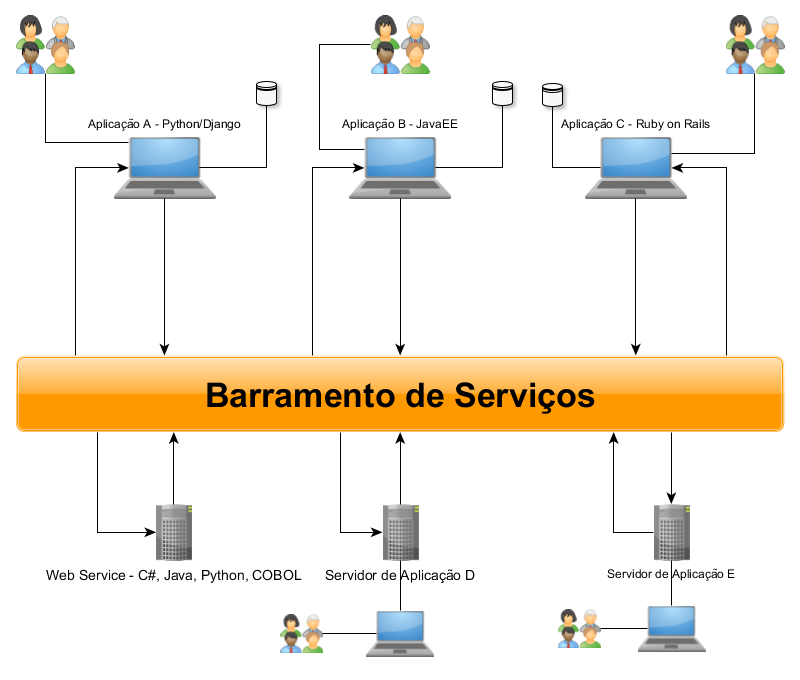
\includegraphics[width=1\textwidth]{figuras/barramento_interoperabilidade.png}
\caption{Interoperabilidade em uma arquitetura baseada no modelo SOA.}
\label{barramento_interoperabilidade}
\end{figure}

A figura acima visa demonstrar a interoperabilidade em uma arquitetura baseada no modelo SOA: é possível inferir que as diversas aplicações fazem a requisição dos serviços disponíveis por meio do uso do barramento de serviços, que também pode ser interpretado como um barramento de aplicações. As aplicações podem ser desenvolvidas utilizando-se tecnologias e paradigmas distintos e a troca de dados entre elas se darão de forma bidirecional via mensagens de requisição e resposta entre as aplicações usuário, que requisitam operações dos serviços, e os serviços, responsáveis por processar as requisições e fornecer a resposta correspondente.

A figura também exibe um fato interessante na arquitetura proposta: não é necessário que um serviço seja apenas um serviço hospedado em um servidor. As aplicações poderão operar tanto em modo \textit{standalone}, sendo executadas de forma independente dos outros serviços ou aplicações, quanto como um serviço para a plataforma virtual ou para outras aplicações que tenham conhecimento da existência e do protocolo de uso deste serviço.

O ESB é uma ferramenta que fornece as funcionalidades do barramento de serviços. Seu uso irá garantir que, sempre que este estiver ativo, as requisições que serão realizadas sempre terão uma resposta, mesmo sendo algo que indique a inatividade do serviço requerido ou a não autorização para acesso à este. Ao adicionar um novo serviço à arquitetura utilizando o ESB, deverão ser especificados tanto os procedimentos quando uma nova requisição for feita quanto aqueles passos que conduzem ao envio de uma resposta de acesso ao serviço especificado, sendo esta resposta advinda do próprio serviço ou uma resposta padrão, também especificada, em caso de falha ou sucesso ao executar a requisição.

Com base nos requisitos essenciais levantados e no estudo realizado sobre o modelo arquitetural SOA, o modelo proposto pode ser visto na imagem abaixo:

\begin{figure}[htb]
\centering
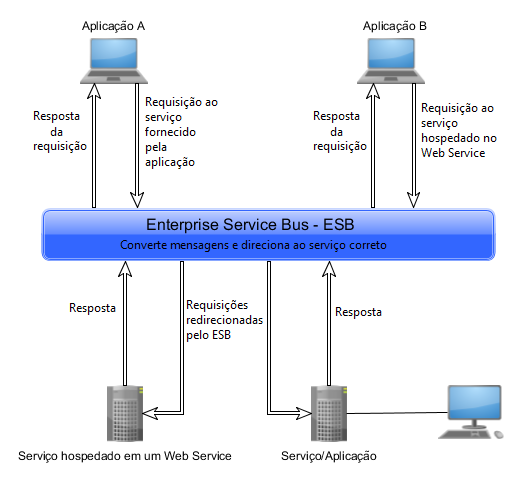
\includegraphics[width=0.7\textwidth]{figuras/uso_esb.png}
\caption{Proposta da arquitetura baseada no modelo SOA com o uso de um ESB.}
\label{uso_esb}
\end{figure}

A comunicação entre aplicações e serviços deverão seguir o padrão de protocolo também definido durante o desenvolvimento deste trabalho de conclusão de curso, para que seja mantida uma regra de execução na troca de informações. O protocolo também facilitará a adição de um novo serviço à arquitetura no que diz respeito aos procedimentos de transformação dos dados e adaptação entre tecnologias e protocolos de transporte e comunicação adotados.

\subsubsection{Ferramentas ESB}
Existem diversas ferramentas deste tipo disponíveis e em uso por grandes organizações, tais como JBoss ESB, Mule ESB, Zato e WSO2 ESB. Para o conhecimento sobre a viabilidade de execução do trabalho aqui proposto, algumas destas ferramentas já foram levantadas, e, sendo o ESB um elemento importante para a implementação aqui proposta, uma análise prévia destas ferramentas já foi realizada. O levantamento feito mostrou que as ferramentas que podem ser utilizadas para a implementação da arquitetura são o JBoss ESB, WSO2 ESB e ErlangMS. Os critérios utilizados foram:

\begin{itemize}
\item Ser uma ferramenta de código aberto e/ou \textit{free};
\item Possuir documentação e tutoriais disponíveis;
\item Facilidade para implantação;
\item Facilidade para uso;
\item Possibilida de de uso de conectores (customizados e existentes);
\item Suporte ao formato de mensagem escolhido para a implementação do protocolo.
\end{itemize}

\subsection{Protocolo de comunicação}
O protocolo de comunicação proposto para que ocorra a troca de dados entre usuários e provedores de serviço é um protocolo geral a ser utilizado por estes e adaptados sempre que necessário, porém não fugindo dos padrões estabelecidos. O protocolo proposto utiliza o modelo REST e, portanto, deve ser aderente à arquitetura deste. Este protocolo foi escolhido por ser de fácil uso, podendo ser implementado em diversas linguagens de programação (principalmente aquelas que são destinadas ao desenvolvimento de plataformas para a web) e em diversos sistemas operacionais. Além disso, o modelo REST utiliza o HTTP como protocolo de transporte, contribuindo para que a comunicação entre diversas aplicações seja realizada de maneira mais estável.

A arquitetura do protocolo REST aceita alguns formatos tais como JSON, CSV e texto simples, como mencionado nos capítulos anteriores. O formato definido para uso neste protocolo é o JSON, por ser um formato que permite a composição da mensagem através de chaves e valores. Assim, quando de posse da mensagem, os valores podem extraídos de acordo com a chave. Estas informações deverão ser publicadas pelo serviço na especificação de suas operações e valores de retorno quando forem acessados.

A fim de permitir o acesso ao serviço, as aplicações devem disponibilizar uma API REST para que os recursos sejam manipulados através das operações. Alguns serviços podem necessitar de autenticação e autorização para acesso ao mesmo, porém outros estarão disponpiveis para uso sem a necessidade de que tais recuros de segurança sejam implementados. Os requisitos de segurança na troca de dados deverão ser planejados em trabalhos futuros.

Desta forma, o fluxo básico do protocolo de comunicação entre os provedores e usuários dos serviços pode ser visto na imagem abaixo: 

\begin{figure}[htb]
\centering
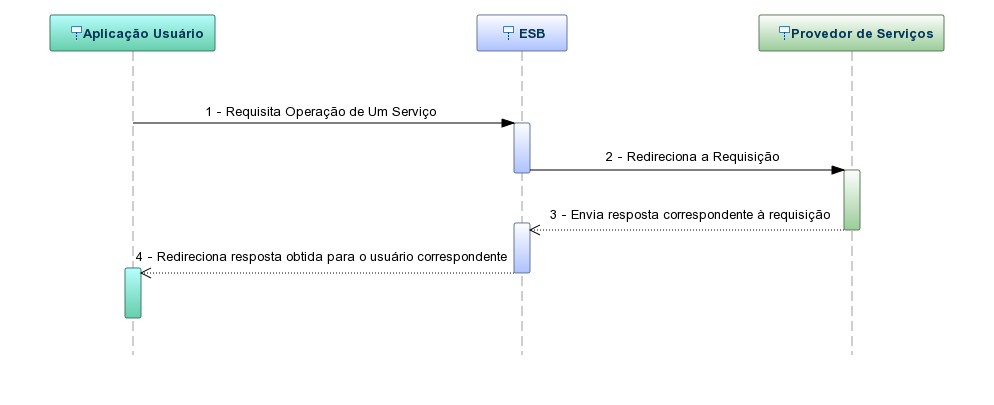
\includegraphics[width=1\textwidth]{figuras/fluxo_basico_protocolo.png}
\caption{Fluxo básico do protocolo de comunicação.}
\label{fluxo_basico_protocolo}
\end{figure}

A imagem exibe o fluxo geral do protocolo de comunicação estabelecido entre o usuário e o provedor de serviços, sendo esta comunicação intermediada pelo ESB: a aplicação que faz uso do serviço requisita que uma operação disponibilizada pelo serviço seja executada, esta requisição, por sua vez, é tratada pelo ESB e redirecionada à aplicação provedora do serviço; a resposta da requisição feita também será intermediada pelo ESB e redirecionada à aplicação que realizou a requisição.

O ESB é o elemento da comunicação que detêm o conhecimento sobre os servidos providos na plataforma e é o ator responsável por realizar a entrega das mensagens de requisição e de resposta dos serviços. Caso necessário, é também uma responsabilidade do ESB, realizar a transformação/adaptação dos formatos das mensagens e dos protocolos usados.

\subsubsection{Formato das Mensagens}
Como anteriormente mencionado, o formato escolhido para a troca de mensagens entre as aplicações será o JSON. A escolha foi realizada pelo fato de este formato de mensagem ser leve, de fácil entendimento e implementação, além de permitir que não seja difícil a recuperação dos dados em qualquer linguagem de programação, bem como pelo ESB.

O formato JSON é baseado em um esquema de chave-valor, onde a chave identifica um atributo, um dado, e o valor é o dado em si, o valor quantitativo ou qualitativo do atributo indicado pela chave. Este formato de mensagem adotado, pode ser tratado na aplicação como uma mensagem JSON ou como uma cadeia de caracteres, a depender da linguagem de programação adotada na construção da plataforma virtual e dos serviços disponibilizados.

Assim, para realizar uma requisição, a aplicação que executa o papel de usuário de um serviço deverá indicar o serviço e a operação desejada, o formato da mensagem (JSON por padrão) e os valores necessários para que o serviço seja executado corretamente, indicados pela API disponibilizada pelo mesmo. Da mesma forma, a resposta também deverá ser gerada em formato JSON, porém a aplicação que prover serviços retorna apenas a resposta da mensagem no padrão chave-valor. Abaixo podem ser visualizados um exemplo de requisição e outro de reposta, ambos em formato JSON.

\begin{figure}[htb]
\centering
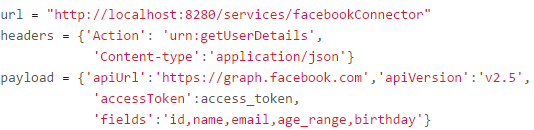
\includegraphics[width=0.8\textwidth]{figuras/mensagem_requisicao.png}
\caption{Exemplo de uma mensagem de requisição de serviço em formato JSON de uma aplicação usuário escrita em Python e Django.}
\label{mensagem_requisicao}
\end{figure}

\begin{figure}[htb]
\centering
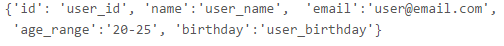
\includegraphics[width=0.8\textwidth]{figuras/mensagem_resposta.png}
\caption{Exemplo de uma mensagem de resposta de requisição em formato JSON.}
\label{mensagem_resposta}
\end{figure}

A primeira imagem exibe os valores necessários para realizar uma requisição ao serviço fornecido pela rede social Facebook através de sua API. Para a chamada do serviço, são necessários a especificação do endereço do serviço, indicado pela \textit{url}; \textit{headers} guarda os valores da operação a ser executada pelo serviço ('\textit{Action}') e o formato da mensagem ('\textit{Content-type}'); os valores necessários para a execução da operação requisitada estão contidos no \textit{payload} também em formato \textit{{'chave':'valor'}}.

As imagens acima mostram apenas exemplos do uso do formato de mensagem JSON para realizar uma requisição e de mensagem obtida como resposta advinda do serviço. Pode-se ver que os valores são correspondentes à uma chave conhecida por ambas as aplicações, permitindo que as aplicações (provedora e usuária de serviços) possam comunicar-se entre si de forma padronizada e conhecida por ambas as partes.
